% !TEX TS-program=xelatex
\documentclass{../../templates/information_retrieval_lab}
\pagestyle{plain}
\begin{document}

% file for general details about your work
\newcommand{\reportAuthor}{Косенко Олександр Володимирович}
%\newcommand{\reportSupervisor}{}
\newcommand{\reportAuthorGroup}{КП-11}
\newcommand{\reportYear}{2025}


\newcommand{\labNo}{1}

\newcommand{\labTopic}{РЕАЛІЗАЦІЯ ТЕОРЕТИКО-МНОЖИННОЇ МОДЕЛІ ПОДАННЯ ДОКУМЕНТІВ}

\thispagestyle{empty}
\setlength{\parindent}{0cm}

\begin{center}
МІНІСТЕРСТВО ОСВІТИ І НАУКИ УКРАЇНИ

НАЦІОНАЛЬНИЙ ТЕХНІЧНИЙ УНІВЕРСИТЕТ УКРАЇНИ

«КИЇВСЬКИЙ ПОЛІТЕХНІЧНИЙ ІНСТИТУТ ІМЕНІ ІГОРЯ СІКОРСЬКОГО»

\vfill

Факультет прикладної математики

Кафедра програмного забезпечення комп’ютерних систем

\vfill

\textbf{Лабораторна робота №\labNo}

з дисципліни «Програмне забезпечення інформаційно-пошукових систем»

тема «\labTopic»
\end{center}

\vfill

{\renewcommand{\arraystretch}{0.7}
\begin{tabularx}{\textwidth}{>{\setlength\hsize{1\hsize}}X >{\setlength\hsize{1\hsize}}X}
&Виконав cтудент\\                                         % & \\
&студент IV курсу групи \reportAuthorGroup\\               % & \\
&\reportAuthor\\                                           % & \rule{2.5cm}{0.25pt}   \\[6pt]
%Керівник:                                                & \\
%\supervisorRegalia                                       & \\
%\supervisorFio                                           & \rule{2.5cm}{0.25pt}   \\[6pt]
%%%%% Якщо у вас є консультант у роботі - розкоментуйте наступні три рядки (а цей - не розкоментовуйте!)
%Консультант:                                             & \\
%\consultRegalia                                          & \\
%\consultFio                                              & \rule{2.5cm}{0.25pt}   \\[6pt]
%Рецензент:                                               & \\
%\reviewerRegalia                                         & \\
%\reviewerFio                                             & \rule{2.5cm}{0.25pt} 
\end{tabularx}
}

\vfill

\centerline{КИЇВ \reportYear}

\setlength{\parindent}{1.25cm}

\pagebreak


\centerline{\textbf{Постановка задачі}}

Реалізувати інформаційно-пошукову систему, що використовує стандартну
булеву модель подання документів, відповідно до наступних вимог:
1. Для реалізації інформаційно-пошукової системи може
використовуватись будь-який стек (мова програмування, фреймворк і
так далі) технологій.

2. Інформаційно-пошукова система може мати будь-який з перелічених
інтерфейсів користувача: консольний, веб, мобільний, настільний.

3. Розроблена інформаційно-пошукова система має використовувати
стандартну булеву модель подання документів.

4. Робота з розробленою інформаційно-пошуковою системою має бути
поділена на наступні етапи:

a. Введення множини індексних термів.

i. Користувач повинен мати можливість ввести будь-яку
невід’ємну кількість індексних термів на свій вибір (хоча б один
індексний терм є обов’язковим).

ii. Допускається (на вибір студента) реалізація введення множини
індексних термів за допомогою її зчитування з файлу будь-якого
формату. У такому випадку, на даному етапі користувач повинен
вводити шлях до цього файлу.

iii. Кожен терм вводиться символами нижнього регістру.

iv. Після закінчення введення множини індексних термів,
користувач повинен автоматично перейти на наступний етап.

b. Введення колекції документів.

i. Користувач повинен мати можливість ввести будь-яку
невід’ємну кількість документів (хоча б один документ у колекції
є обов’язковим).

ii. Допускається (на вибір студента) реалізація введення колекції
документів за допомогою її зчитування з окремих текстових
файлів, розміщених у певній директорії (один текстовий файл =
один документ). У такому випадку, на даному етапі користувач
вводить шлях до директорії з файлами.

iii. Документи складаються з термів, розділених пробілами (без
знаків пунктуації), та написаних символами лише нижнього
регістру.

iv. Після закінчення введення, користувач автоматично переходить
на наступний етап.

c. Виконання пошукових запитів.

i. На даному етапі користувач вводить пошуковий запит і
переглядає його результати.

ii. Пошуковий запит вводиться у кон’юнктивній або диз’юнктивній
нормальній формі, відповідно до варіанту студента (див. далі).

iii. Після виконання пошукового запиту, користувач повинен
залишатися на цьому ж етапі, з можливістю ввести новий
пошуковий запит.

Варіант студента визначається за порядковим номером студента у списку
його групи. Якщо номер студента є непарним числом, то пошуковий запит
повинен вводитися у кон’юнктивній нормальній формі. Якщо номер студента є
парним числом, то пошуковий запит повинен вводитися у диз’юнктивній
нормальній формі.

\centerline{\textbf{Хід роботи}}

Лістинг 1. Програмний код допоміжних структур

\lstinputlisting[language=C, style=minimalist]{../program/src/data_structures/string.h}

Структура \texttt{string} призначена для зберігання змінних строкових рядків разом з їх розміром. Структура \texttt{str\_arr\_list} призначена для зберігання списків рядків, заснованих на масивах. Структура \texttt{uint\_arr\_list} призначена для зберігання списків беззнакових цілих чисел.

Лістинг 2. Програмний код функцій для роботи з допоміжними структурами

\lstinputlisting[language=C, style=minimalist]{../program/src/data_structures/string.c}

Лістинг 3. Програмний код структур даних для пошуку інформації

\lstinputlisting[language=C, style=minimalist]{../program/src/information_retrieval/data_structures.h}

Структура \texttt{inverted\_index} призначена для зберігання інвертованого індексу та включає список термів та відповідних їм документів (точніше їх індексів).

Структура \texttt{CNF\_query} призначена для зберігання запиту у кон'юнктивній нормальній формі. Вона включає список структур \texttt{disjunction}, призничених для зберігання окремих диз'юнктів. Диз'юнкти включають список структур \texttt{term\_query} - окремих термів.

Лістинг 4. Програмний код пошуку інформації

\lstinputlisting[language=C, style=minimalist]{../program/src/information_retrieval/data_structures.c}

Функція \texttt{inverted\_index\_heap\_sort\_terms} реалізує алгоритм heap sort для сортування індексу за термами в алфавітному порядку. Дане сортування має найкращу, середню та найгіршу складності відповідно $\Omega(n\log n)$, $\Theta(n\log n)$ та $O(n\log n)$ та використання пам'яті $O(1)$, що є перевагою над такими методами, як quick sort (використання пам'яті $O(\log n)$) та merge sort (використання пам'яті $O(n)$), особливо враховуючи те, що на практиці в індексі має зберігатись велика кількість термів.

Функція \texttt{inverted\_index\_get\_postings} повертає список документів, що містять даний терм. Пошук виконується алгоритмом бінарного пошуку, що має складність $O(\log n)$. Хоча він і поступається складності пошуку в хеш-таблиці, зберігання термів у хеш-таблиці вимагає більше пам'яті для того, щоб колізії були достатньо рідкісними.

Функція \texttt{query\_from\_str} перетворює введений користувачем рядок на запит.

Функція \texttt{index\_document\_iterator} заповнює інвертований індекс документами (точніше, їх числовими індексами). Документи зчитуються по одному з допомогою функції-ітератора. Після цього за словами, що містяться в документі, здійснюється пошук списку термів. У разі існування до списку додається індекс документа.

Функція \texttt{uint\_arr\_list\_union} приймає два списки цілих чисел (відсортовані за зростанням) та повертає їх об'єднання (відсортоване за зростанням).

Функція \texttt{uint\_arr\_list\_complement} приймає список цілих чисел та довжину повного списку документів та повертає список цілих чисел, що є доповненням вхідного списку.

Функція \texttt{inverted\_index\_retrieve} проводить пошук за запитом у інвертованому індексі. При цьому спочатку обчислюється наближений розмір списків документів, отриманих в окремих диз'юнктах як сума довжин списків відповідних термів (у разі заперечення терму довжина списку оцінюється як різниця довжини повного списку документів та списку терму). Після цього утворюється список, що відповідає найменшій наближеній довжині як об'єднання списків термів відповідного диз'юнкту. Після цього даний список може лише зменшуватись, отже при перетині з іншим диз'юнктом відбувається маркування елементів списку. На початку елементи помічені на видалення. Якщо елемент належить списку терму або не належить списку заперечного терму, він помічається для збереження. Після проходження диз'юнкту зі списку видаляються всі не помічені на збереження елементи.

Лістинг 5. Програмний код меню програмного застосунку

\lstinputlisting[language=C, style=minimalist]{../program/src/main.c}

Функція \texttt{inverted\_index\_from\_terms} утворює інвертований індекс з рядка, що містить терми, розділені пробілами.

Функція \texttt{main} містить реалізацію користувацького меню.

\centerline{\textbf{Результати роботи}}

Для демонстрації результату створимо документи поділивши на чатини статтю з Вікіпедії (\url{https://en.wikipedia.org/wiki/C_(programming_language)}), прибравши з тексту все що не є літерами та пробілами та звівши всі літери до малих.

\begin{figure}[H]
    \centering
    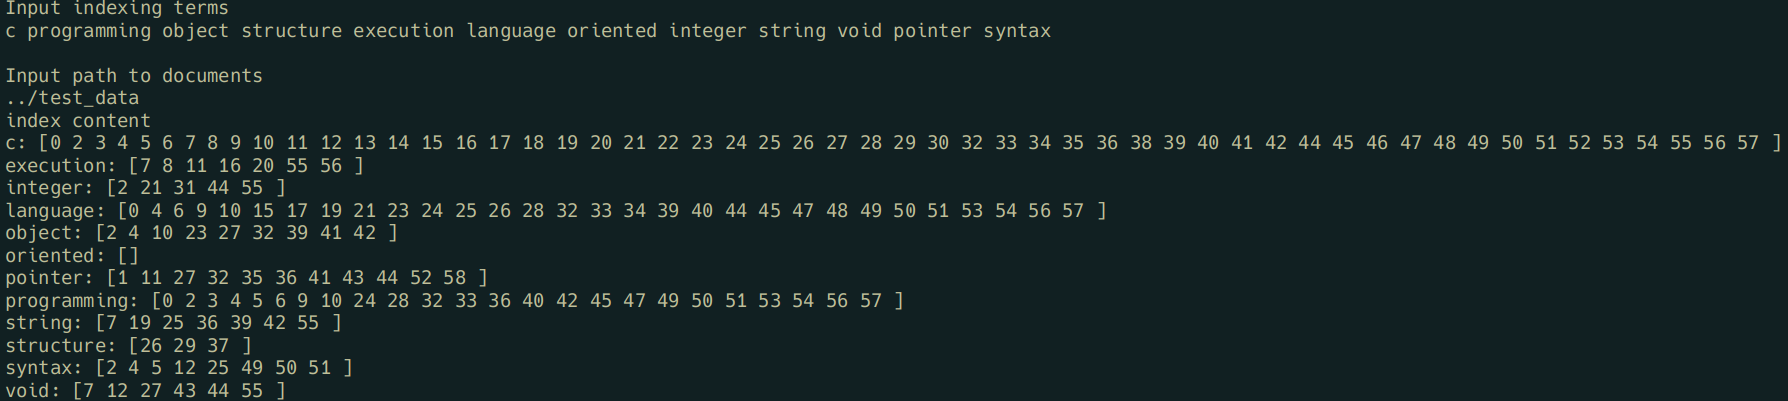
\includegraphics[width=\textwidth]{img/screen0.png}
    \caption{Введення термів та шляху до документів}
\end{figure}

\begin{figure}[H]
    \centering
    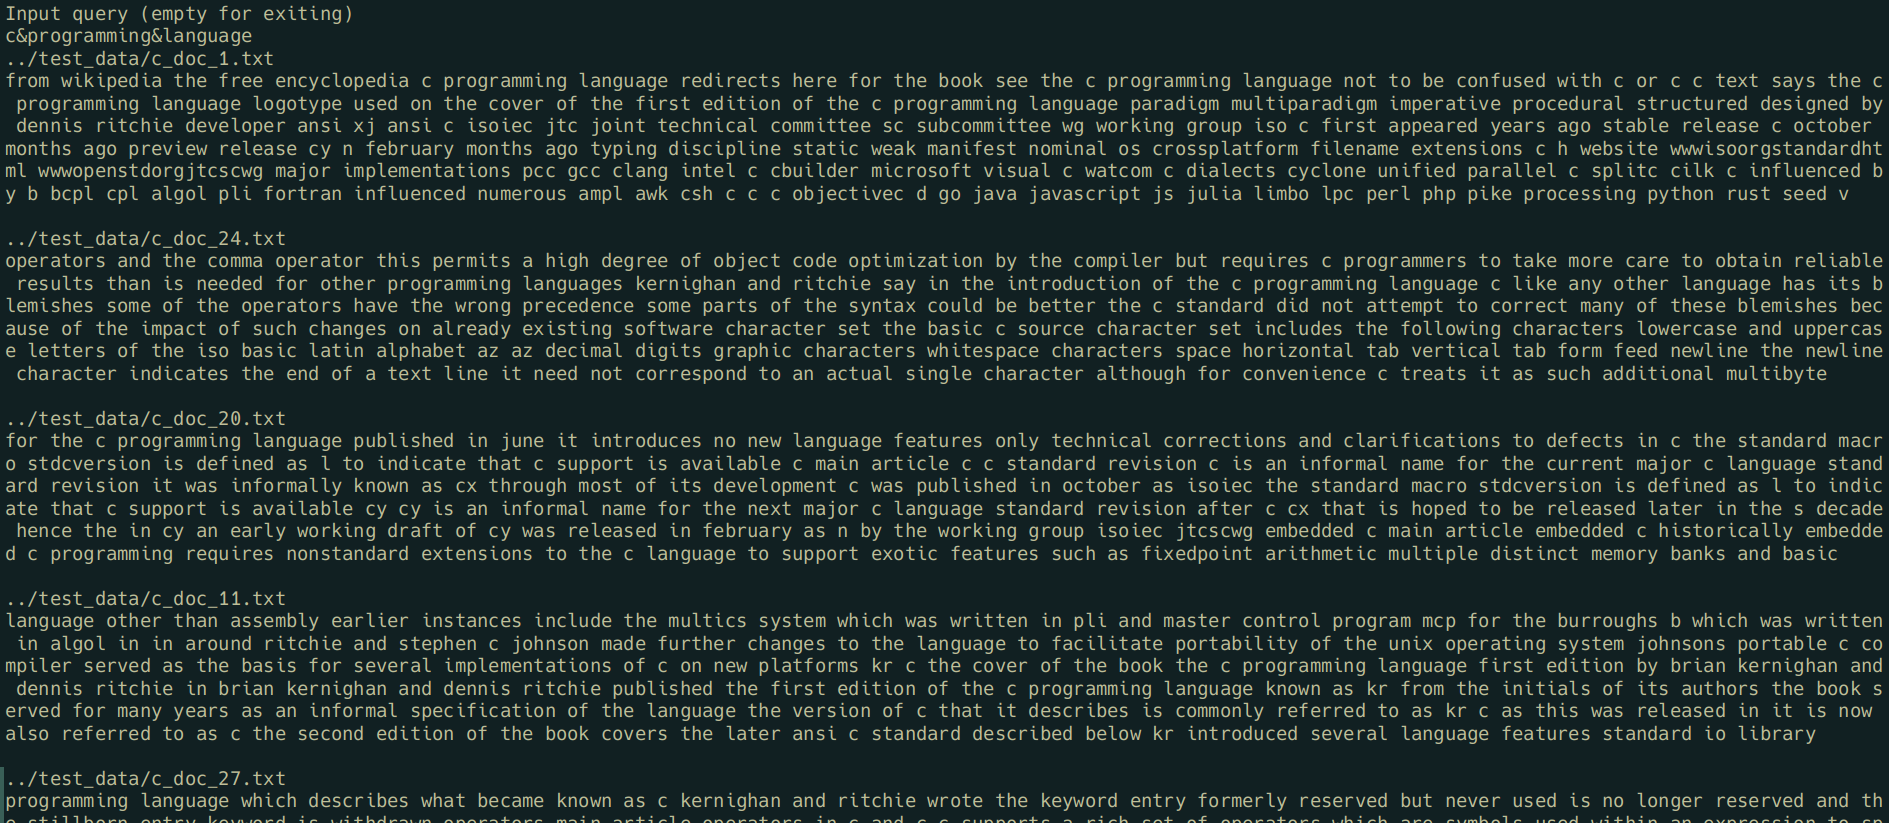
\includegraphics[width=\textwidth]{img/screen1.png}
    \caption{Приклад пошуку}
\end{figure}

\begin{figure}[H]
    \centering
    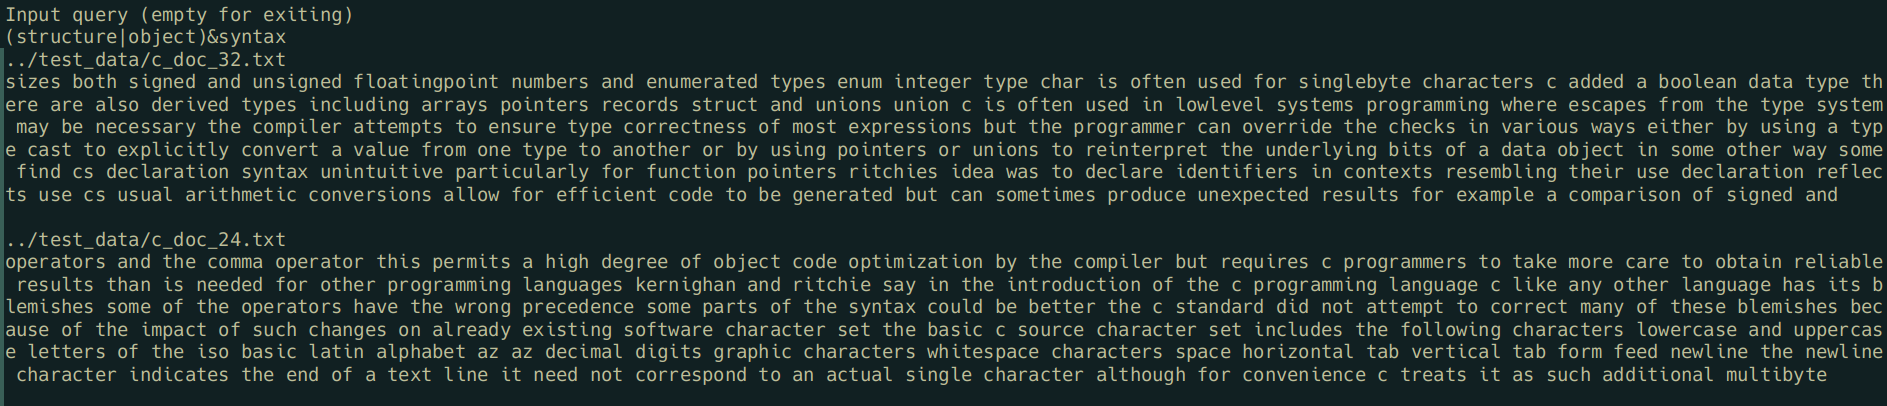
\includegraphics[width=\textwidth]{img/screen2.png}
    \caption{Приклад пошуку з диз'юнкцією}
\end{figure}

\begin{figure}[H]
    \centering
    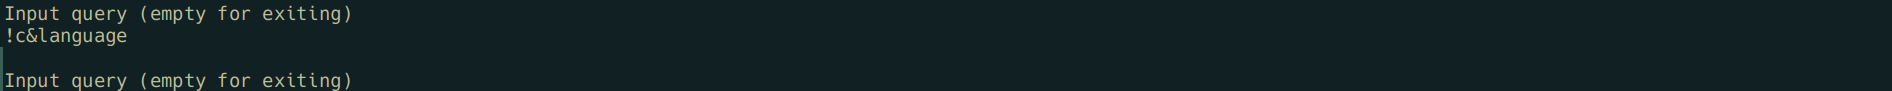
\includegraphics[width=\textwidth]{img/screen3.png}
    \caption{Приклад пошуку з запереченням (порожній)}
\end{figure}

\begin{figure}[H]
    \centering
    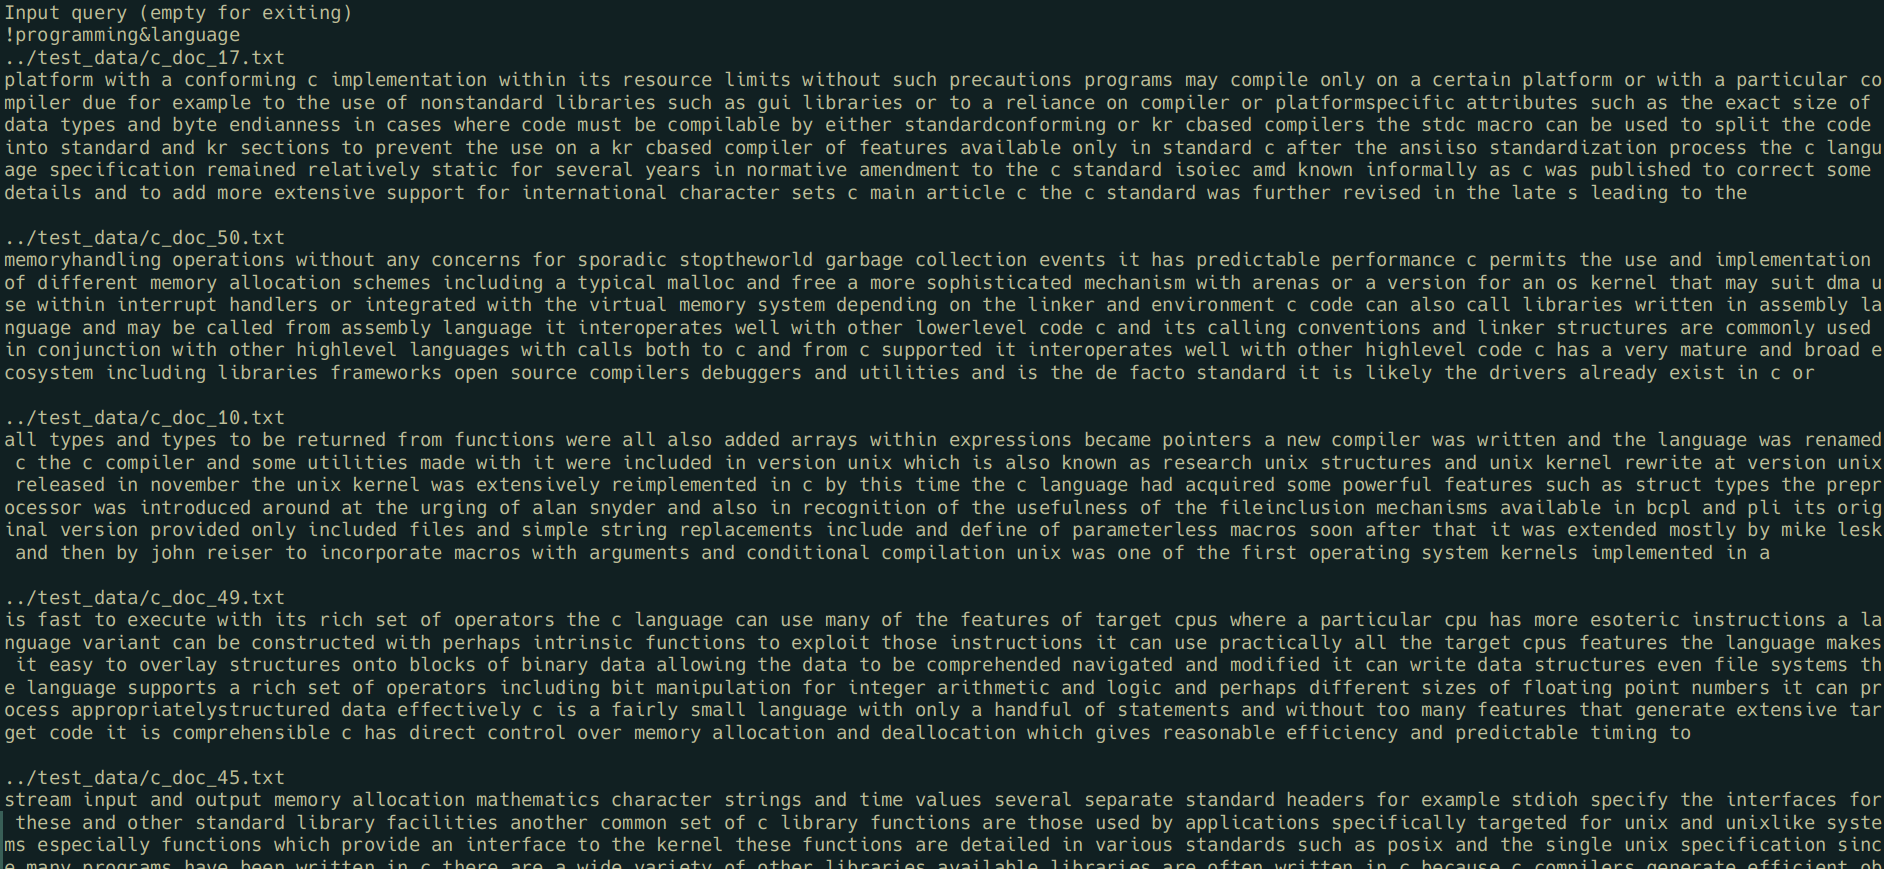
\includegraphics[width=\textwidth]{img/screen4.png}
    \caption{Приклад пошуку з запереченням}
\end{figure}

\textbf{Висновки:} у ході виконання даної лабораторної роботи розглянуто пошук з використанням теоретико-множинної моделі подання документів. Створено інвертований індекс та здійснено пошук за цим індексом з використанням запитів у кон'юнктивній нормальній формі. Використано оптимізації пошуку, такі як використання властивостей сортованих списків, сортування з $O(1)$ використанням пам'яті та $O(n\log n)$ використанням часу, сортування диз'юнктів за їх прогнозованим розміром тощо.

\end{document}
